% 18-09-2024

\chapter{Espacios Topológicos}

\begin{definicion}
    Un \textbf{espacio topológico} es una par $(X, \cc{T})$, donde $X \neq \emptyset$ es un conjunto y $\cc{T}\subset\cc{P}(X)$ es una familia de subconjuntos de $X$.

    \begin{enumerate}
        \item[\textbf{(\hypertarget{A1}{A1})}] $\emptyset, X \in \cc{T}$.
        \item[\textbf{(\hypertarget{A2}{A2})}] Si $\{U_i\}_{i\in I} \subset \cc{T}$, entonces $\bigcup\limits_{i\in I} U_i \in \cc{T}$.
        \item[\textbf{(\hypertarget{A3}{A3})}] Si $U_1, U_2 \in \cc{T}$, entonces $U_1 \cap U_2 \in \cc{T}$.
    \end{enumerate}

    A la familia $\cc{T}$ se le llama \textbf{topología} en el conjunto $X$. A los elementos de $\cc{T}$ se les llama \textbf{abiertos} en el espacio topológico $(X, \cc{T})$.
\end{definicion}

\vspace*{0.5cm}

\begin{observacion}
    De \hyperlink{A1}{\textbf{(A1)}} podemos concretar que si $U_1, \dots, U_k \in \cc{T}$, entonces \smash{$\bigcap\limits_{i=1}^{\infty}U_i \in \cc{T}$}.
    En general, si $\{U_i\}_{i=1}^{\infty}\in \cc{T}$, entonces $\bigcup\limits_{i=1}^{\infty}$ no tiene por qué ser abierto.
\end{observacion}

\begin{ejemplo}\ 
    \begin{itemize}
        \item \textbf{Topología trivial:} Sea $X \neq \emptyset$, $\cc{T}_t = \{\emptyset, X\} \Rightarrow (X, \cc{T}_t)$ es un e.t\footnote{A partir de ahora notaremos así a un espacio topológico}.
        \item \textbf{Topología discreta:} Sea $X \neq \emptyset$, $\cc{T}_{disc}= \cc{T}_{D} = \cc{P}(X) \Rightarrow (X, \cc{T}_D)$ es un e.t.
        \item \textbf{Topología del punto incluido:} Sea $X \neq \emptyset$, $x_0\in X$ $\cc{T}_{x_0} = \{\emptyset\}\cup \{U \subset X : x_0 \in U\} \Rightarrow (X, \cc{T}_{x_0})$ es un e.t.
        \item \textbf{Topología cofinita:} (o topología de los complementos finitos) Sea $X \neq \emptyset$, $\cc{T}_{CF} = \{\emptyset\}\cup\{U\subset X : X \setminus U \text{ es finito}\} \Rightarrow (X, \cc{T}_{CF})$ es un e.t.
        \begin{gather*}
            X \setminus \left(\bigcup\limits_{i\in I}U_i\right) = \bigcap\limits_{i\in I}(X \setminus U_i) \text{(intersección de finitos es finito)}\\
            X \setminus (U_1 \cap U_2) = (X\setminus U_1) \cup (X \setminus U_2)\text{(unión de finitos es finito)}
        \end{gather*}
        \item \textbf{Topología conumerable:} (o topología de los complementos numerables) Sea $X \neq \emptyset$, $\cc{T}_{CF} = \{\emptyset\}\cup\{U\subset X : X \setminus U \text{ es numerable}\} \Rightarrow (X, \cc{T}_{CF})$ es un e.t.
        \item $\bb{R}$, $ \cc{T}=\{\emptyset, \bb{R}, \bb{Q}, \bb{R}\setminus \bb{Q}\}, \Rightarrow (\bb{R}, \cc{T})$ es un e.t. 
        \item \textbf{Topología de Sierpinski:} $X=\{a,b\}$, $\cc{T}=\{\emptyset, \{a\}, X\} \Rightarrow (X, \cc{T})$ es un e.t.
        \item \textbf{Topología de Sorgenfrey:} $X=\bb{R}$, $\cc{T}_S$, $U\in \cc{T}_S \sii \forall x \in U \ \  \exists \veps > 0 \text{ tal que } [x, x+\veps) \subset U$. (es un caso particular del punto incluido, $\cc{T}_a$).
    \end{itemize}
\end{ejemplo}

\newpage

\begin{observacion}
    En $X=\{x\}$ solo existe una topología, $\cc{T}=\{\emptyset, \{x\}\}$ (todas las topologías son la misma).
\end{observacion}

\begin{ejercicio}
    Determinar todas las topologías en un conjunto con 2 elementos.\\
    % Hay 4: trivial, discreta y punto incluido con cada elemento

    Consideramos $X=\{a,b\}$. Las topologías posibles son:
    \begin{itemize}
        \item Trivial: $\cc{T}_t=\{\emptyset, X\}$
        \item Discreta: $\cc{T}_{disc}=\cc{P}(X)$
        \item Punto incluido (a): $\cc{T}_a = \{\emptyset, \{a\}, X\}$
        \item Punto incluido (b): $\cc{T}_b = \{\emptyset, \{b\}, X\}$
    \end{itemize}
    \endsquare
\end{ejercicio}

\begin{ejercicio}
    Sea $(X, \cc{T})$ e.t. Demostrar que $\cc{T}=\cc{T}_{disc} \sii \{x\}\in \cc{T}\ \  \forall x \in X$. 
    % Implicación derecha es trivial
    \begin{itemize}
        \item[$\Rightarrow$)] Si $\cc{T} = \cc{T}_{disc}$, como $\{x\}\in \cc{P}(X) \ \ \forall x \in X$, se tiene que $\{x\}\in \cc{T}_{disc} = \cc{T}$.
        \item[$\Leftarrow$)] Tenemos $\{x\} \in \cc{T} \ \ \forall x \in X$. Consideramos $U \in \cc{P}(X)$ un subconjunto cualquiera de $X$. Podemos expresar $U=\bigcup\limits_{i\in I} \{x_i\}$, donde $\{x_i\} \in X \ \ \forall i \in I$. Por la propiedad \apuntar{A2} tenemos $U \in \cc{T}$. Como $U$ era un subconjunto arbitrario de $X$, tenemos $\cc{T}=\cc{T}_{disc}$.
    \end{itemize}
    \endsquare
\end{ejercicio}

\section{Topología métrica. La topología usual de $\bb{R}^n$}

\begin{definicion}
    Un \textbf{espacio métrico} es un par $(X, d)$ donde $X \neq \emptyset$ es un conjunto y $d: X \times X \rightarrow \bb{R}$ es una aplicación que verifica:
\end{definicion}

\begin{enumerate}
    \item [\textbf{(\hypertarget{D1}{D1})}] $d(x, y) \geq 0$\ \ $\forall x,y \in X$. Además, $d(x,y)= 0 \sii x=y$.
    \item [\textbf{(\hypertarget{D2}{D2})}] (simetría) $d(x,y)=d(y,x)$ $\forall x, y, \in X.$
    \item [\textbf{(\hypertarget{D3}{D3})}] (desigualdad triangular) $d(x,z) \leq d(x,y) + d(y,z)$\ \ $\forall x,y,z \in X$
\end{enumerate}

A la aplicación $d$ la llamaremos \textbf{distancia}.

\begin{ejercicio}
    % (D2) + (D3) + 2ª parte de (D1) se deduce 1ª parte de (D1) luego $d:X \times X \rightarrow [0, \infty)$
    Demostrar que a partir de las propiedades \hyperlink{D2}{\textbf{(D2)}}, \hyperlink{D3}{\textbf{(D3)}} y la segunda parte de \hyperlink{D1}{\textbf{(D1)}} se puede deducir la primera parte de \hyperlink{D1}{\textbf{(D1)}}, y como consecuencia se tiene $d:X \times X \rightarrow [0, \infty)$.\\

    Para cualesquiera $x,y \in X$, tenemos:
    \begin{gather*}
        0 \overset{\apuntar{D1}{(2)}}{=} d(x,x) \overset{\apuntar{D3}}{\leq} d(x,y) + d(y,x) \overset{\apuntar{D2}}{=} d(x,y) + d(x,y) = 2 d(x,y)
    \end{gather*}
    De donde podemos deducir
    \begin{gather*}
        d(x,y) \geq 0 \Rightarrow d:X \times X \rightarrow [0, \infty)
    \end{gather*}

    \endsquare
        
\end{ejercicio}

\begin{definicion}
    $(X,d)$ e.m. $x \in X$, $r >0$, se definen:

    \begin{itemize}
        \item La \textbf{bola (abierta)} de centro $x$ y radio $r$ como 
        \begin{gather*}
            B(x, r) = \{y \in X : d(x,y) < r\} \subset X
        \end{gather*}
        \item La \textbf{bola cerrada} de centro $x$ y radio $r$ como 
        \begin{gather*}
            \overline{B}(x, r) = \{y \in X : d(x,y) \leq r\} \subset X
        \end{gather*}
        \item La \textbf{esfera} de centro $x$ y radio $r$ como 
        \begin{gather*}
            S(x, r) = \{y \in X : d(x,y) = r\} \subset X
        \end{gather*}
    \end{itemize}
\end{definicion}

Algunas propiedades que se deducen de la definición anterior son:
\begin{itemize}
    \item $\overline{B}(x, r) = B(x,r) \cup S(x,r)$
    \item $S(x,r) = \overline{B}(x, r) \setminus B(x,r)$
    \item Si $s<r$, entonces $\overline{B}(x, x) \subset B(x,r)$
\end{itemize}

\begin{ejemplo}(Espacio euclídeo $\bb{R}^n$)
    En $\bb{R}^n$ consideramos la \textbf{distancia usual}, 
    \begin{gather*}
        d(x,y) = \|x-y\| = \sqrt{\sum\limits_{i=1}^2(x_i-y_i)^2}
    \end{gather*}

    Al espacio métrico $(\bb{R}^n, d )$ lo denominaremos \textbf{Espacio Euclídeo}.

    \begin{itemize}
        \item Si $n=1$, $d(x,y) = |x-y|$,,  %Arreglar
        \begin{align*}
            B(x,r) &= (x-r, x+r)\\
            \overline{B}(x,r) &= [x-r, x+r]\\
            S(x,r) &= \{x,y\}
        \end{align*}
        
        \item En $n=2$ tenemos
        
        \vspace*{0.25cm}

        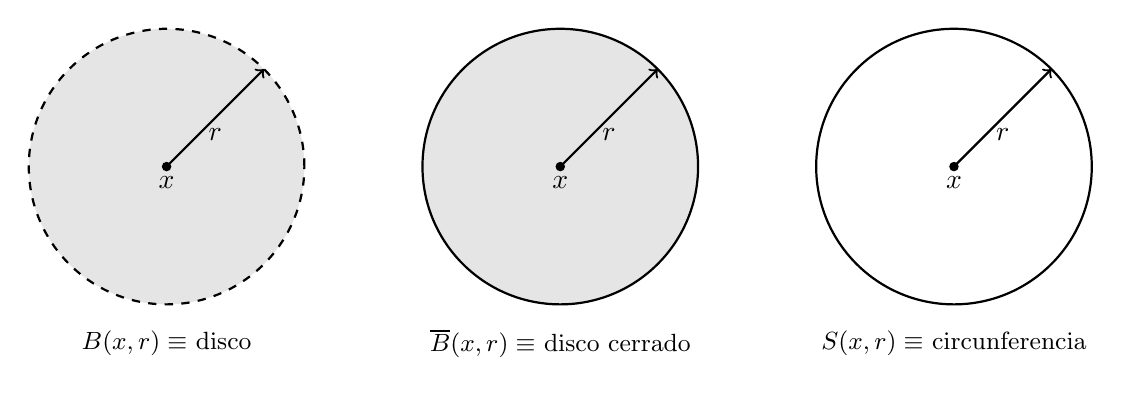
\begin{tikzpicture}
            \centering

            \def\radius{1.75}
            \def\incolor{gray!20}
            \def\angulo{45}

            % Desactiva los caracteres conflictivos
            \shorthandoff{>} % Para poner puntas de flecha

            \filldraw[dashed, fill=\incolor, thick] (-5,0) circle (\radius);
            \filldraw (-5,0) circle (1.5pt)  node[below] {$x$};
            \draw[thick, ->] (-5,0) -> ({-5+sin(\angulo)*\radius}, {cos(\angulo)*\radius}) node[midway, below] {$r$};
            \node at (-5,-2.25) {\small{$B(x,r) \equiv$ disco}};

            \filldraw[fill=\incolor, thick] (0,0) circle (\radius);
            \filldraw (0,0) circle (1.5pt)  node[below] {$x$};
            \draw[thick, ->] (0,0) -> ({sin(\angulo)*\radius}, {cos(\angulo)*\radius}) node[midway, below] {$r$};
            \node at (0,-2.25) {\small{$\overline{B}(x,r) \equiv$ disco cerrado}};

            \draw[thick] (5,0) circle (\radius);
            \filldraw (5,0) circle (1.5pt)  node[below] {$x$};
            \draw[thick, ->] (5,0) -> ({5+sin(\angulo)*\radius}, {cos(\angulo)*\radius}) node[midway, below] {$r$};
            \node at (5,-2.25) {\small{$S(x,r) \equiv$ circunferencia}};
        \end{tikzpicture}

        \item En $n=3$ tenemos:
        
        \vspace*{0.25cm}

        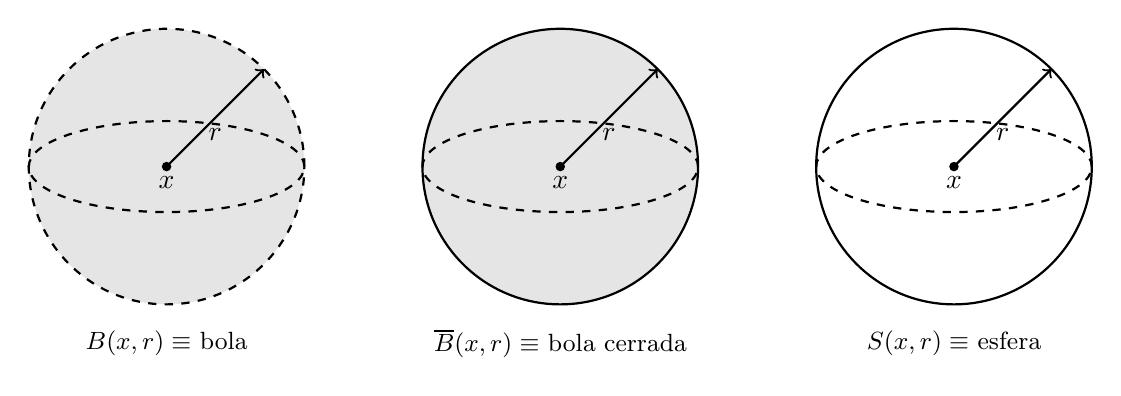
\begin{tikzpicture}
            \centering

            \def\radius{1.75}
            \def\incolor{gray!20}
            \def\angulo{45}

            % Desactiva los caracteres conflictivos
            \shorthandoff{>} % Para poner puntas de flecha

            \filldraw[dashed, fill=\incolor, thick] (-5,0) circle (\radius);
            \draw[dashed, thick] (-5,0) ellipse [x radius=\radius, y radius=0.33*\radius];
            \filldraw (-5,0) circle (1.5pt)  node[below] {$x$};
            \draw[thick, ->] (-5,0) -> ({-5+sin(\angulo)*\radius}, {cos(\angulo)*\radius}) node[midway, below] {$r$};
            \node at (-5,-2.25) {\small{$B(x,r) \equiv$ bola}};

            \filldraw[fill=\incolor, thick] (0,0) circle (\radius);
            \draw[dashed, thick] (0,0) ellipse [x radius=\radius, y radius=0.33*\radius];
            \filldraw (0,0) circle (1.5pt)  node[below] {$x$};
            \draw[thick, ->] (0,0) -> ({sin(\angulo)*\radius}, {cos(\angulo)*\radius}) node[midway, below] {$r$};
            \node at (0,-2.25) {\small{$\overline{B}(x,r) \equiv$ bola cerrada}};

            \draw[thick] (5,0) circle (\radius);
            \draw[dashed, thick] (5,0) ellipse [x radius=\radius, y radius=0.33*\radius];
            \filldraw (5,0) circle (1.5pt)  node[below] {$x$};
            \draw[thick, ->] (5,0) -> ({5+sin(\angulo)*\radius}, {cos(\angulo)*\radius}) node[midway, below] {$r$};
            \node at (5,-2.25) {\small{$S(x,r) \equiv$ esfera}};
        \end{tikzpicture}
    \end{itemize}
\end{ejemplo}

\begin{ejemplo}
    $X \neq \emptyset$ se define la \textbf{distancia discreta} como 
    \begin{align*}
        d_{disc}(x,y) &=
        \left\{ 
        \begin{array}{ccc}
            0 & \text{si} & x=y\\
            1 & \text{si} & x\neq y
        \end{array}
        \right. 
    \end{align*}
    Con la distancia así definida tenemos:
    \begin{align*}
        B(x,y) &=
        \left\{ 
        \begin{array}{ccc}
            X & \text{si} & r>1\\
            \{x\} & \text{si} & r \leq 1
        \end{array}
        \right. \\\\
        \overline{B}(x,y) &=
        \left\{ 
        \begin{array}{ccc}
            X & \text{si} & r \geq 1\\
            \{x\} & \text{si} & r < 1
        \end{array}
        \right.\\\\
        S(x,y) &=
        \left\{ 
        \begin{array}{ccc}
            X \setminus \{x\} & \text{si} & r =1 \\
            \emptyset & \text{si} & r \neq 1\\
        \end{array}
        \right.
    \end{align*}
\end{ejemplo}


\begin{ejemplo}\
    \begin{itemize}
        \item Si $d$ es una distancia en $X$ y $\lambda > 0$, entonces $\lambda \cdot d : X \times X \rightarrow [0,\infty)$ también es una distancia y $B_{\lambda d}(x,r) = B_d(x, \dfrac{r}{\lambda})$
        \item Sean $d$ y $\tilde{d}$ distancias en $X$ y $d \leq \tilde{d}$, entonces $B_d(x,r) \geq B_{\tilde{d}}(x,r)$
    \end{itemize}
\end{ejemplo}

\begin{definicion}
    $(X,d)$ e.m. Un subconjunto $U \subset X$ se dice \textbf{abierto métrico} si $U=\emptyset$ o si $\forall x \in U, \ \ \exists r > 0$ tal que $B(x,r) \subset U$.
\end{definicion}

\begin{prop} %proposicion
    Si $(X,d)$ es un espacio métrico, entonces 
    \begin{gather*}
        \cc{T}_d=\{U \subset X : U \text{ es un abierto métrico en }(X,d)\} \subset \cc{P}(X)
    \end{gather*}
    es una topología en $X$ que llamamos la \textbf{topología métrica} en $(X,d)$.

    \begin{proof}\
        \begin{enumerate}[label=(A\arabic*)]
            \item $\emptyset$, $X\in \cc{T}_d$ trivialmente.
            \item Sea $\{U_i\}_{i\in I}\subset \cc{T}_d$. ¿$\bigcup\limits_{i\in I}U_i \in \cc{T}_d$?
            
            Si $\bigcup\limits_{i\in I}U_i = \emptyset \Rightarrow \bigcup\limits_{i\in I}U_i \in \cc{T}_d$.

            Supongamos $\bigcup\limits_{i\in I}U_i \neq \emptyset$. Sea $x \in \bigcup\limits_{i\in I}U_i \Rightarrow \exists i \in I : x \in U_i \in \cc{T}_d \Rightarrow \exists r>0 : B(x,r) \subset U_i \subset \bigcup\limits_{i\in I}U_i \Rightarrow \bigcup\limits_{i\in I}U_i\in \cc{T}$.

            \item Sean $U_1, U_2 \in \cc{T}_d$. ¿$U_1 \cap U_2 \in \cc{T}_d$?
            
            Si $U_1 \cap U_2 = \emptyset$ se verifica.

            Supongamos $U_1 \cap U_2 \neq \emptyset$. Entonces puedo considerar $x\in U_1 \cap U_2 \Rightarrow \exists r_1,r_2>0: B(x,r_1)\subset U_1$ y $B(x,r_2)\subset U_2 \Rightarrow B(x, \min\{r_1, r_2\}) \subset U_1 \cap U_2$
        \end{enumerate}
    \end{proof}

\end{prop}

\begin{definicion}
    Se llama \textbf{topología usual de $\bb{R}^n$}, $\cc{T}_u$, a la topología métrica en $\bb{R}^n$ con la distancia usual, es decir,
    $U \subset \bb{R}^n$ es abierto en $(\bb{R}^n, \cc{T}_u)$ si $U=\emptyset$ o si $\forall x \in U \ \ \exists r>0 : B(x,r) \subset U$.
\end{definicion}

\begin{prop}
    $(X,d)$ e.m. Se cumplen:
    \begin{enumerate}
        \item[(i)] Las bolas abiertas en $(X,d)$ son abiertos.
        \item[(ii)] Todo abierto no vacío en $(X,d)$ se puede escribir como unión de bolas abiertas y como unión de bolas cerradas.
    \end{enumerate}


    \begin{proof}\
        \begin{enumerate}
            \item[(i)] Sea $x\in X$, $r>0$, ¿$B(x, r)\in \cc{T}_d$?
            
            Sea $y \in B(x,r) \Rightarrow d(x,y)<r \Rightarrow \exists \veps>0 : d(x,y) + \veps <r \Rightarrow B(y, \veps)\subset B(x,r)$. Para ver esta última implicación tenemos que si tomamos un $z \in B(y, \veps)\Rightarrow d(x,z) \leq d(x,y) + d(y,z) < d(x,y) + \veps < r \Rightarrow z \in B(x,r)$. %TODO: añadir dibujo de la demostración

            \begin{center}
                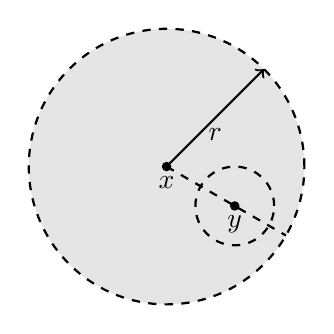
\begin{tikzpicture}
                    \centering
        
                    \def\radius{1.75}
                    \def\incolor{gray!20}
                    \def\angulo{45}
        
                    % Desactiva los caracteres conflictivos
                    \shorthandoff{>} % Para poner puntas de flecha
        
                    \filldraw[dashed, fill=\incolor, thick] (0,0) circle (\radius);
                    \filldraw (0,0) circle (1.5pt)  node[below] {$x$};
                    \draw[thick, ->] (0,0) -> ({sin(\angulo)*\radius}, {cos(\angulo)*\radius}) node[midway, below] {$r$};
                    \def\angulo{120}
                    \draw[thick, dashed] (0,0) -- ({sin(\angulo)*\radius}, {cos(\angulo)*\radius});

                    \filldraw ({sin(\angulo)*1}, {cos(\angulo)*1}) circle (1.5pt)  node[below] {$y$};

                    \def\radius{0.5}
                    \draw[dashed, thick] ({sin(\angulo)*1}, {cos(\angulo)*1}) circle (\radius);
        
                \end{tikzpicture}
            \end{center}
            
            \item[(ii)] Sea $U \in \cc{T}_d \Rightarrow \forall x \in U \ \ \exists r_x >0$ tal que $B(x,r_x)\subset U \Rightarrow U = \bigcup\limits_{x\in U}B(x, r_x) = \bigcup\limits_{x\in U}\overline{B}\left(x, \frac{r_x}{2}\right)$.
            
        \end{enumerate}
    \end{proof}
\end{prop}

\begin{coro}
    En $(X,d)$ tenemos 
    \begin{gather*}
        \cc{T}_d=\{\emptyset\}\cup\{U \subset X : U \text{ es unión de bolas abiertas}\}
    \end{gather*}
\end{coro}

\begin{ejemplo}\
    \begin{itemize}
        \item $(X,d)$ e.m. En general, no todo abierto es una bola. Pir ejemplo la unión de bolas no concéntricas.
        \item No todo conjunto en $(\bb{R}^n, \cc{T}_u)$ es abierto. Por ejemplo $\{x\}\subset \bb{R}^n$ no es abierto.
        \item En $(\bb{R}, \cc{T}_u)$ los únicos intervalos abiertos (topológicamente) son los intervalos abiertos, es decir, los del tipo $\bb{R}=(-\infty, +\infty)$, $(a,b)$ con $a<b$, $(-\infty, a)$ y $(b, +\infty)$.
        \item En $(X, d)$, en general la intersección infinita de abiertos no es abierto. Por ejemplo, $\bigcap\limits_{n\in \bb{N}}\left(\frac{-1}{n}, \frac{1}{n}\right) = \{0\}$ que no es abierto.
        \item $X\neq \emptyset$, $\cc{T}_{d_{disc}}=\cc{T}_{disc}$ (la topología asociada a la distancia discreta es la distancia discreta).
    \end{itemize}
\end{ejemplo}

\begin{definicion}
    Sean $X\neq \emptyset$ y $d_1, d_2$ distancias en $X$. Decimos que $d_1$ y $d_2$ son \textbf{equivalentes} si existen $a,b>0$ tal que 
    \begin{gather*}
        a \cdot d_1(x,y) \leq d_2(x,y) \leq b \cdot d_1(x,y) \ \ \ \forall x,y \in X
    \end{gather*}
\end{definicion}

\begin{prop}
    Si $d_1, d_2$ son distancias en $X \neq \emptyset$ y existe $a>0$ tal que $a \cdot d_1(x,y) \leq d_2(x,y) \ \ \ \forall x,y \in X$, entonces $\cc{T}_{d_1} \subset \cc{T}_{d_2}$. En particular, si $d_1$ y $d_2$ son equivalentes, entonces $\cc{T}_{d_1} = \cc{T}_{d_2}$.


    \begin{proof}
        Sea $U\in \cc{T}_{d_1}$, $U \neq \emptyset$, ¿$U\in \cc{T}_{d_2}$?

        Sea $x \in U \in \cc{T}_{d_1} \Rightarrow \exists r>0: B_{d_1}(x,r)\subset U$. Como $a \cdot d_1 \leq d_2 \Rightarrow B_{d_2}(x,a\cdot r)\subset B_{d_1}(x,r)$. Para verlo sea $y\in B_{d_2}(x,a\cdot r) \Rightarrow d_2(x,y)<a\cdot r \Rightarrow a \cdot d_1(x,y)<r \Rightarrow y \in B_{d_1}(x,r)$. Por tanto $B_{d_1}(x,r)\subset U \Rightarrow U \in \cc{T}_{d_2}\Rightarrow T_{d_1}\subset \cc{T}_{d_2}$.
        
    \end{proof}
\end{prop}

\begin{definicion}
    Un e.t. $(X,\cc{T})$ se dice \textbf{metrizable} si existe una distancia $d$ en $X$ tal que $\cc{T}= \cc{T}_d$.
\end{definicion}

\begin{ejemplo}\ 
    \begin{itemize}
        \item $(\bb{R}^n, \cc{T}_u)$ es metrizable.
        \item $(X, \cc{T}_{disc})$ es metrizable.
    \end{itemize}
\end{ejemplo}

\begin{ejercicio}
    Si $(X,\cc{T})$ es un e.t. metrizable, entonces cumple la condición de Hausdorff:
    \begin{gather*}
        \forall x,y\in X, x\neq y, \ \ \exists U,V \in \cc{T} : U \cap V = \emptyset
    \end{gather*}
\end{ejercicio}

\begin{ejemplo}\
    \begin{itemize}
        \item $(X,\cc{T}_t)$ no es metrizable si $\#X>2$ (cardinal del conjunto) ya que no verifica la condición de Hausdorff.
        \item $(X, \cc{T}_{x_0})$ no es metrizable por la misma razón (ya que la intersección de cualesquiera dos abiertos va a contener a $x_0$).
        \item $(X, \cc{T}_{CF})$ no es metrizable si $X$ es infinito (aplicar las leyes de morgan para la intersección).
        \item $(X, \cc{T}_{CN})$ no es metrizable si $X$ no es numerable.
        \item $(\bb{R}, \{\emptyset, \bb{R}, \bb{Q}, \bb{R}\setminus \bb{Q}\})$.
        \item La topología de Sierpinski tampoco es metrizable (ya que el único abierto que contiene a $b$ es el total).
        \item La topología de Sorgenfrey $(\bb{R}, \cc{T}_S)$ cumple la propiedad de Hausdorff.
    \end{itemize}
\end{ejemplo}


